\chapter{Risultati}

\begin{itemize}
\item Introduzione teorica
\item Osservazione sull'influenza dell'errore fem (particolare nel caso RRRR sarebbe da verificare)
\item Notare la superconvergenza (come da teoria?)
\end{itemize}

\begin{figure}[!htbp]
        \centering%
        \subfigure[DDDD]%
          {\label{fig: convDDDD}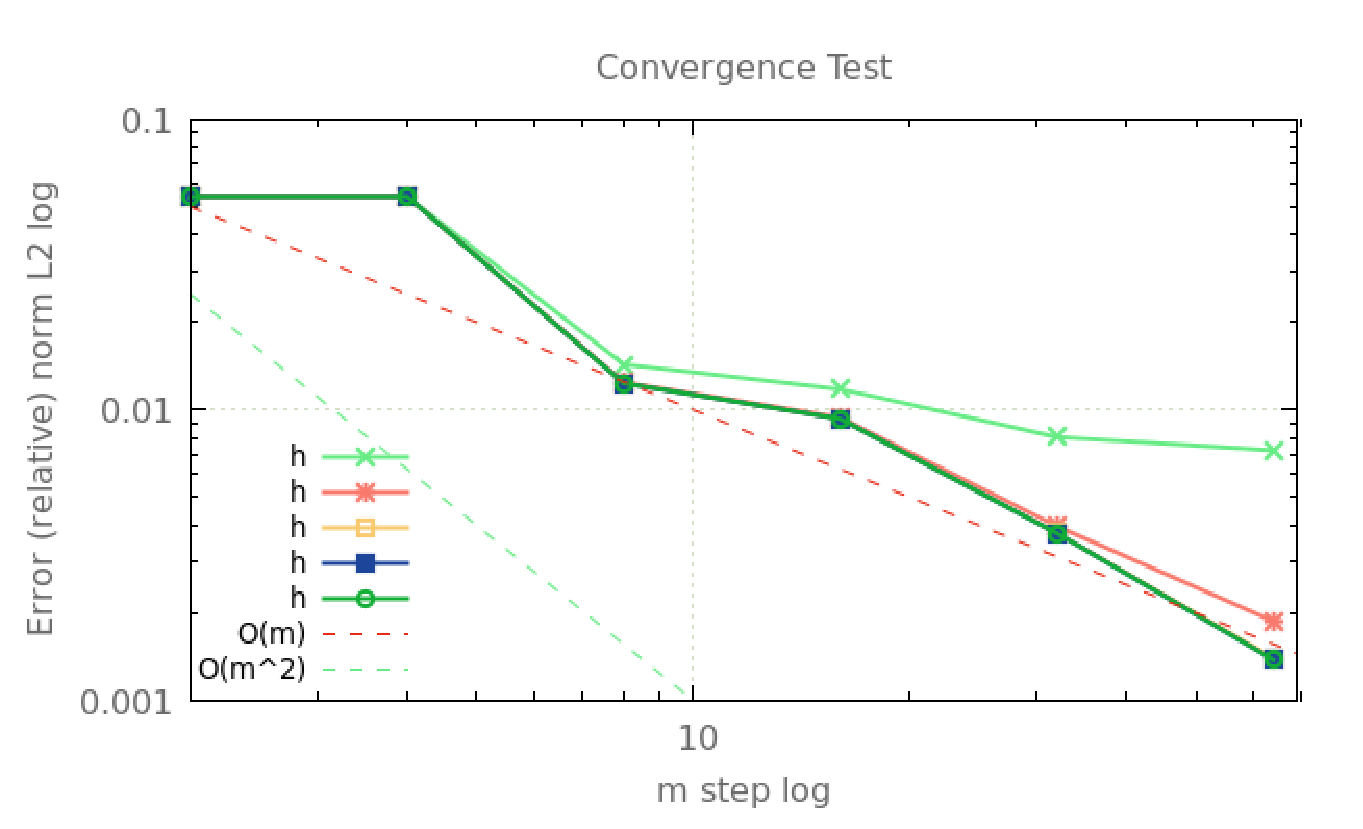
\includegraphics[scale=0.25]{Convergenze/DDDD_ADR.eps}}\qquad
        \subfigure[DRDR]%
          {\label{fig:convDRDR}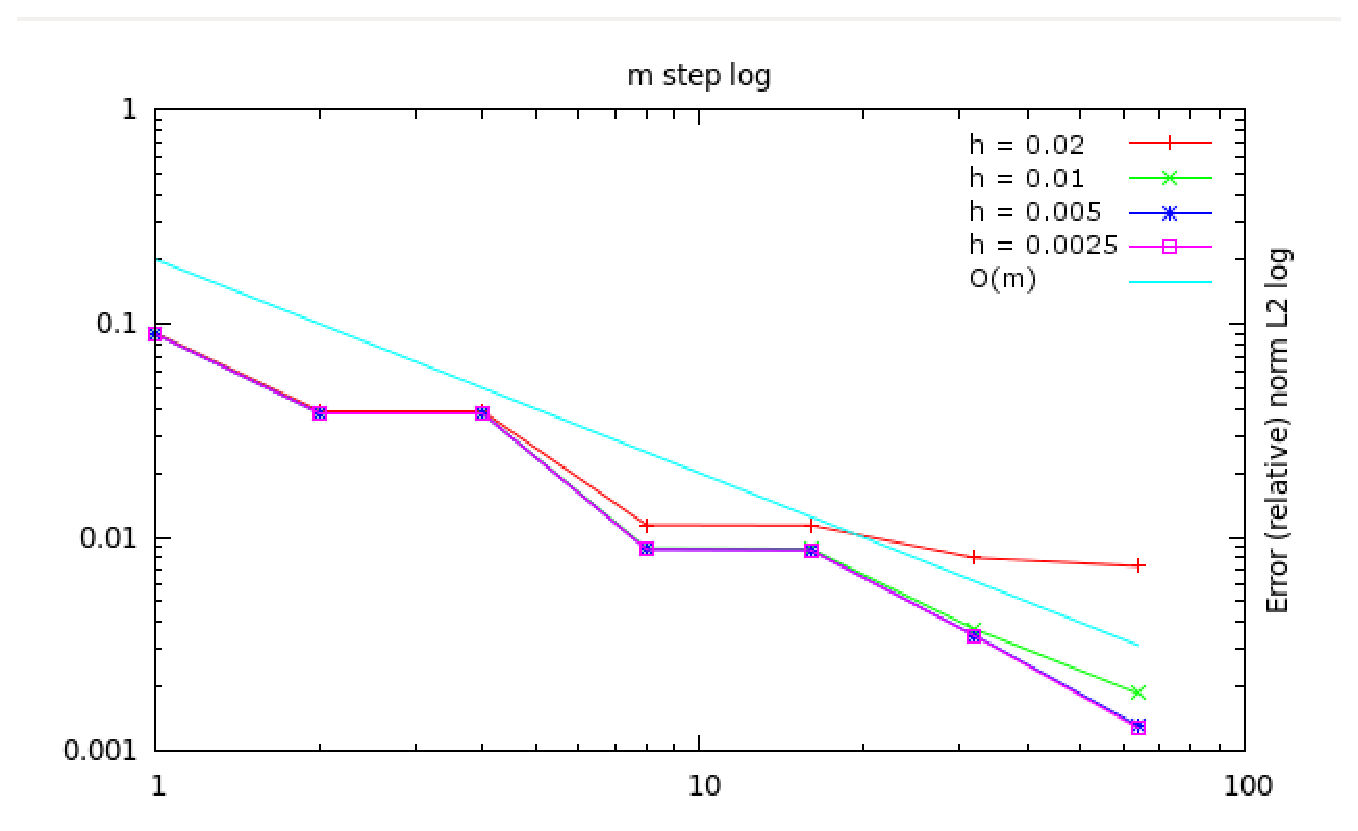
\includegraphics[scale=0.25]{Convergenze/DRDR.eps}}\qquad
		\subfigure[RRRR]%
          {\label{fig:convRRRR}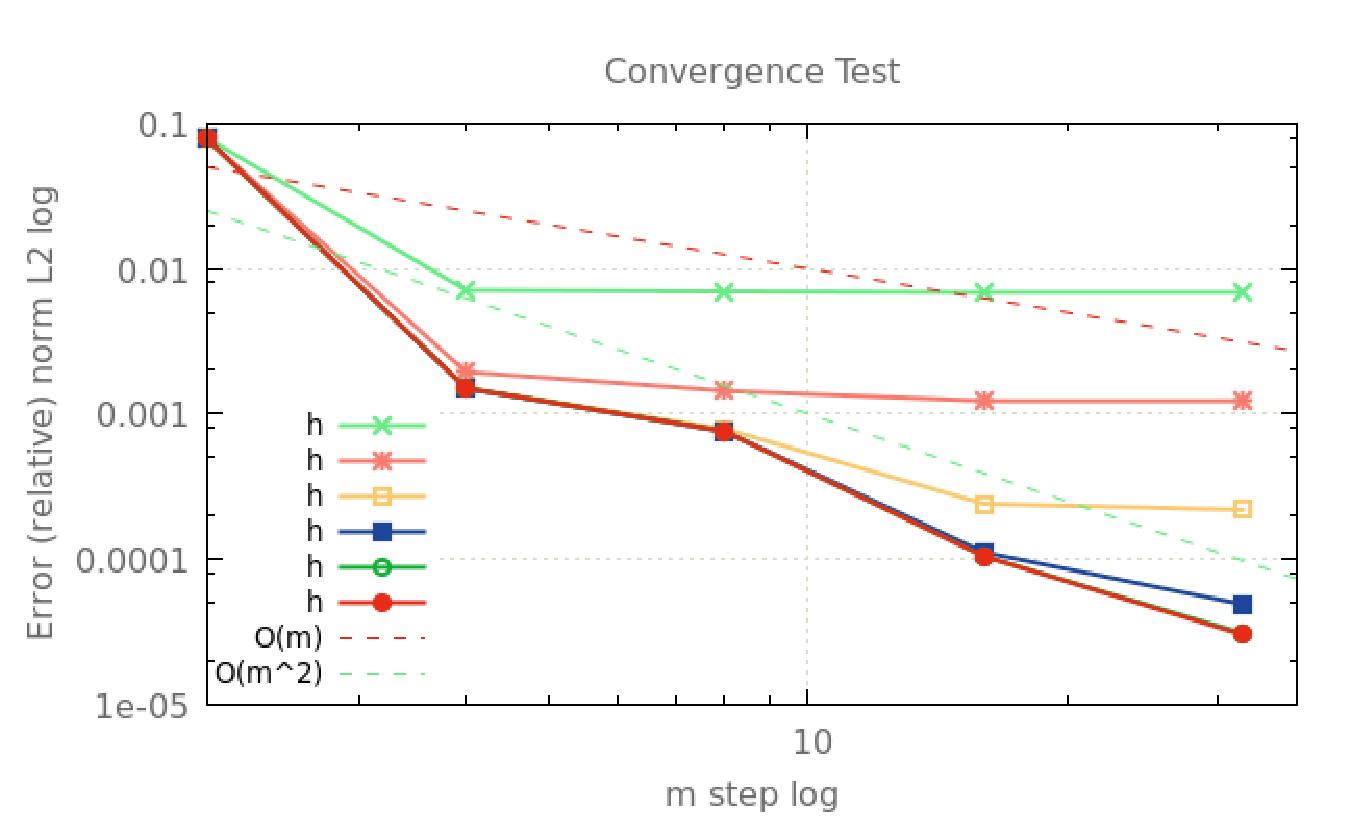
\includegraphics[scale=0.25]{Convergenze/RRRR.eps}}\qquad
        \label{fig: convergenze}
        \caption{Convergenze casi test}
\end{figure}

\begin{itemize}
\item Confronto gradi di libert\`a spesi e errore norma L2
\item Tempo di assemblaggio problema
\end{itemize}
\begin{figure}[!h]
\centering
          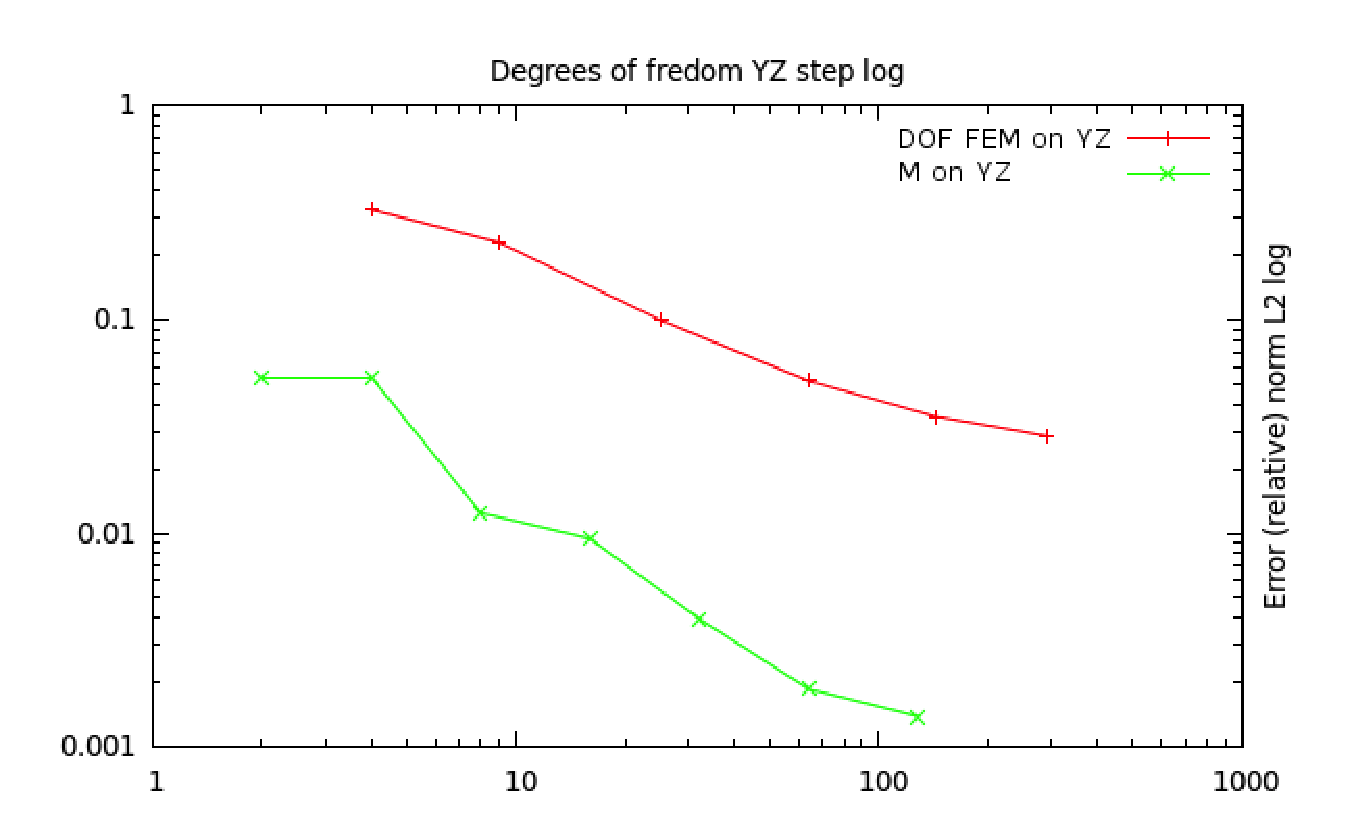
\includegraphics[scale=0.25]{Convergenze/ConfrontoDOF.eps}\qquad
        \caption{ Confronto DOF}
        \label{fig: Confronto DOF}
\end{figure}

\begin{itemize}
\item Presentazione del caso test
\item Osservazione sull'aggiunta progressiva di modi (sempre pi\`u frequenze vengono considerate e l'approssimazione cresce)
\item Commento sui risultati 3D
\end{itemize}

\begin{figure}[!htbp]
        \centering%
        \subfigure[m=9.]%
          {\label{fig: slice9}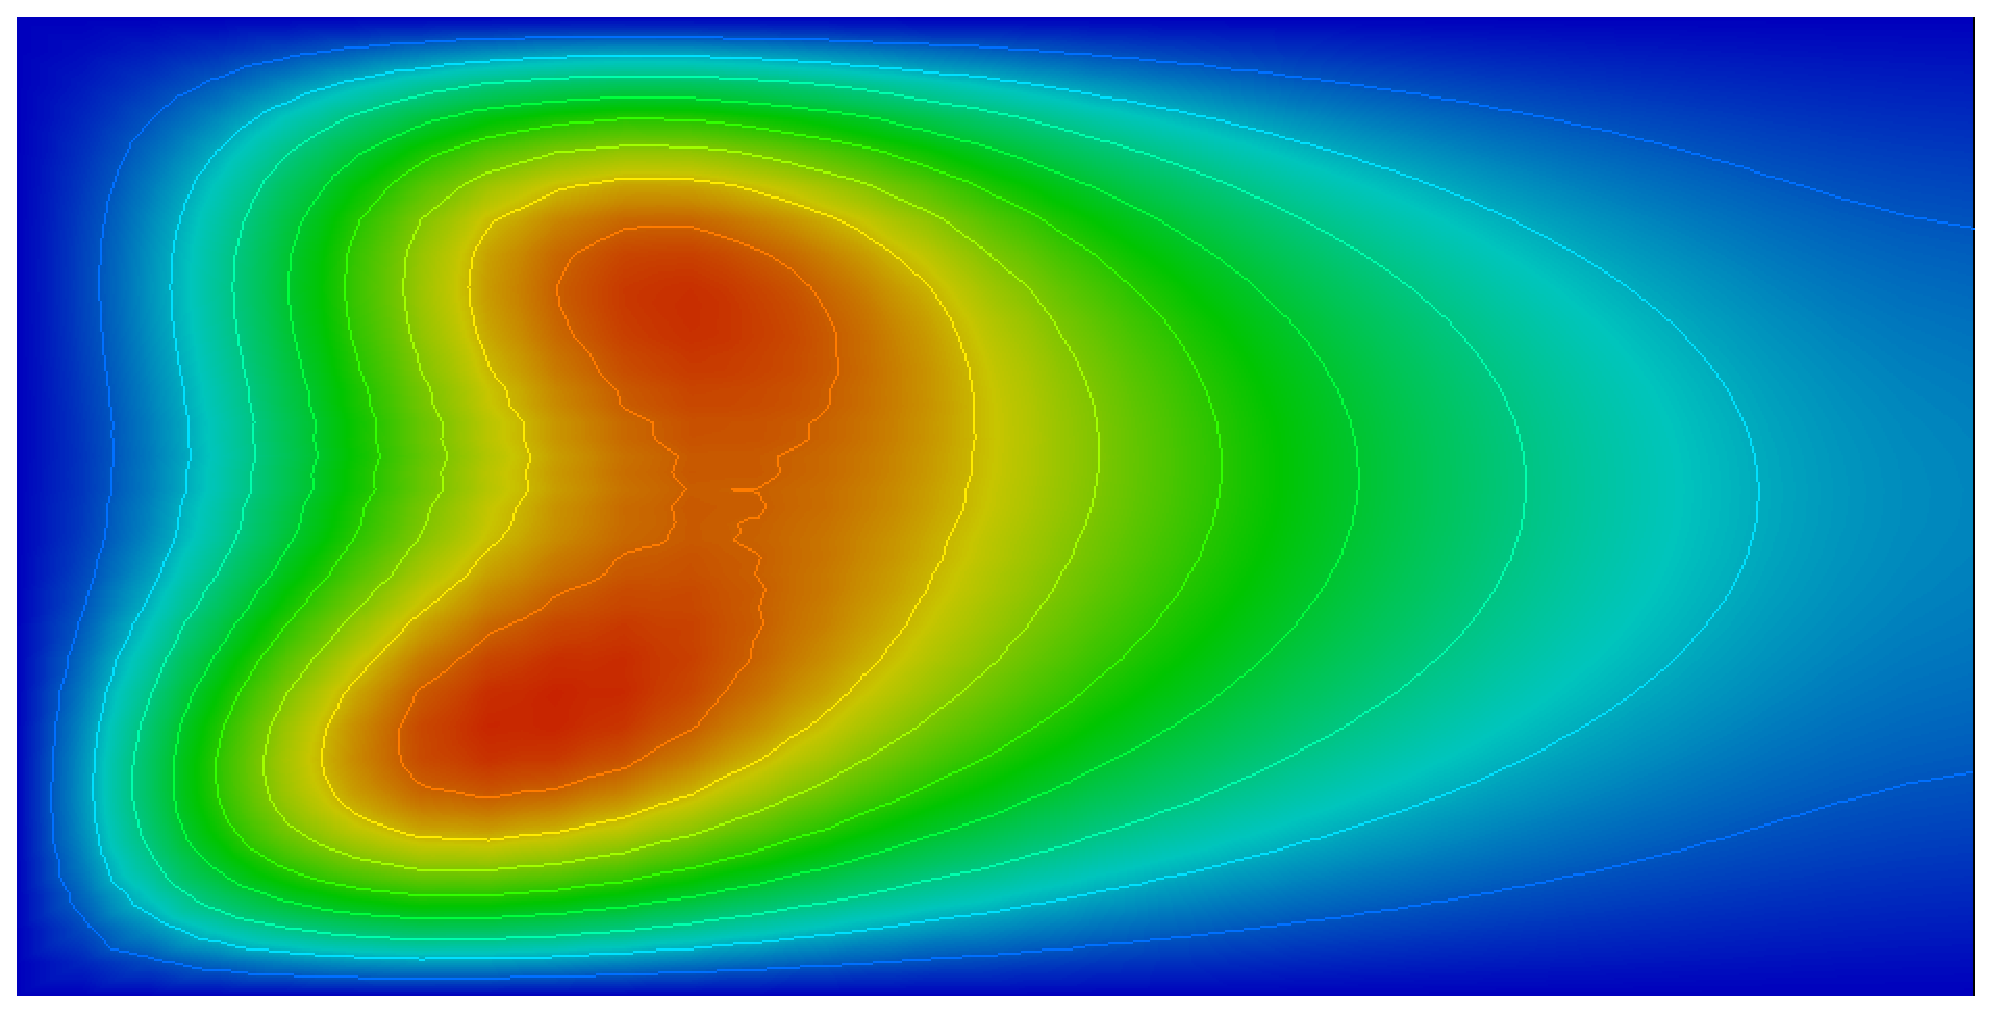
\includegraphics[scale=0.15]{DDDD_ADR/HiMod9slice.eps}}\qquad
        \subfigure[m=16.]%
          {\label{fig:slice16}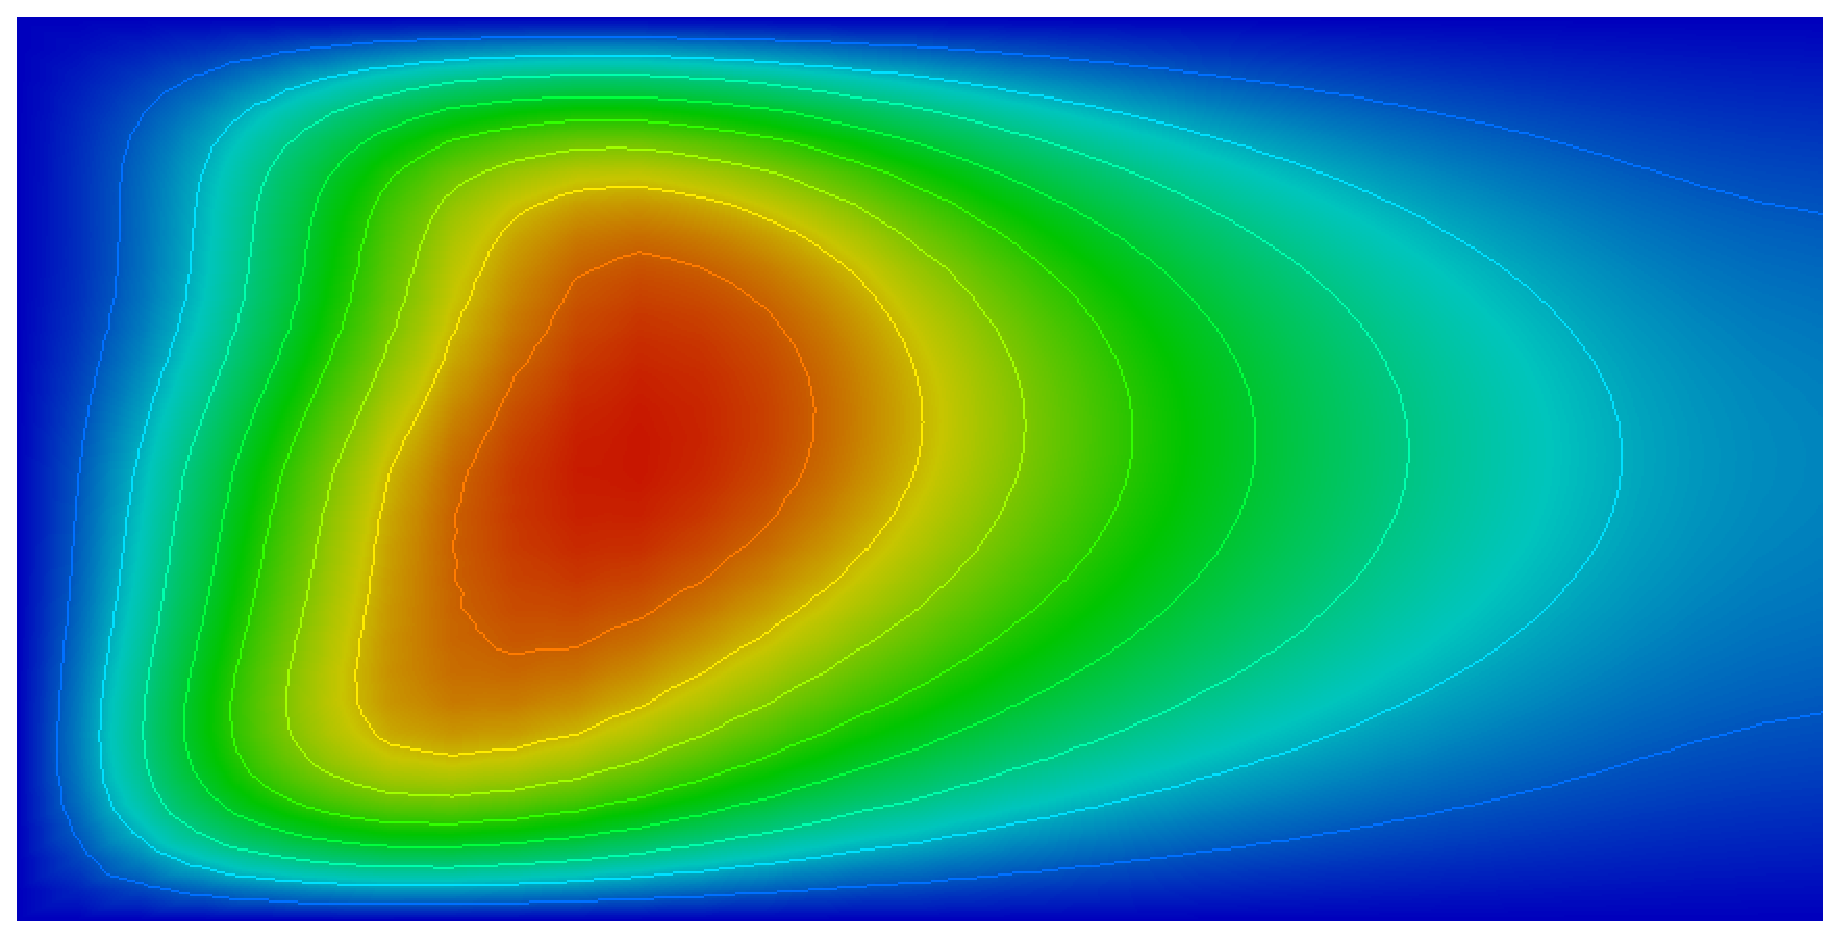
\includegraphics[scale=0.15]{DDDD_ADR/HiMod16slice.eps}}\qquad
		\subfigure[m=25.]%
          {\label{fig:slice25}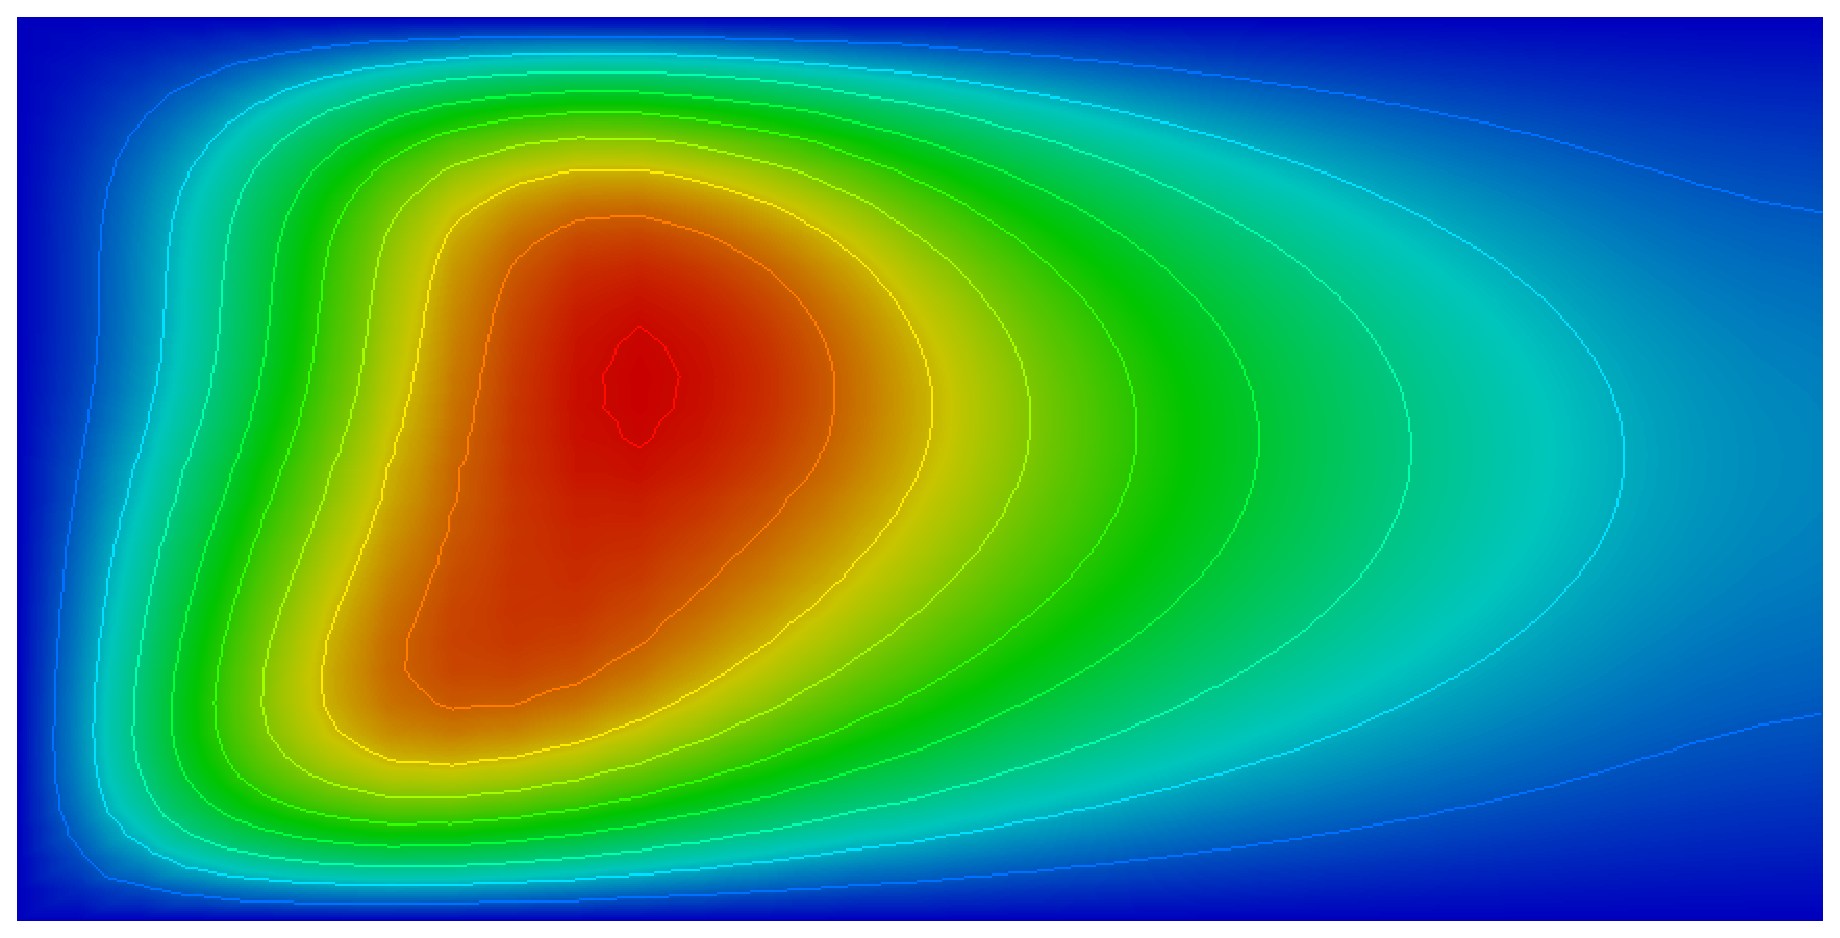
\includegraphics[scale=0.15]{DDDD_ADR/HiMod25slice.eps}}\qquad
          \subfigure[FEM.]%
          {\label{fig:sliceFEM}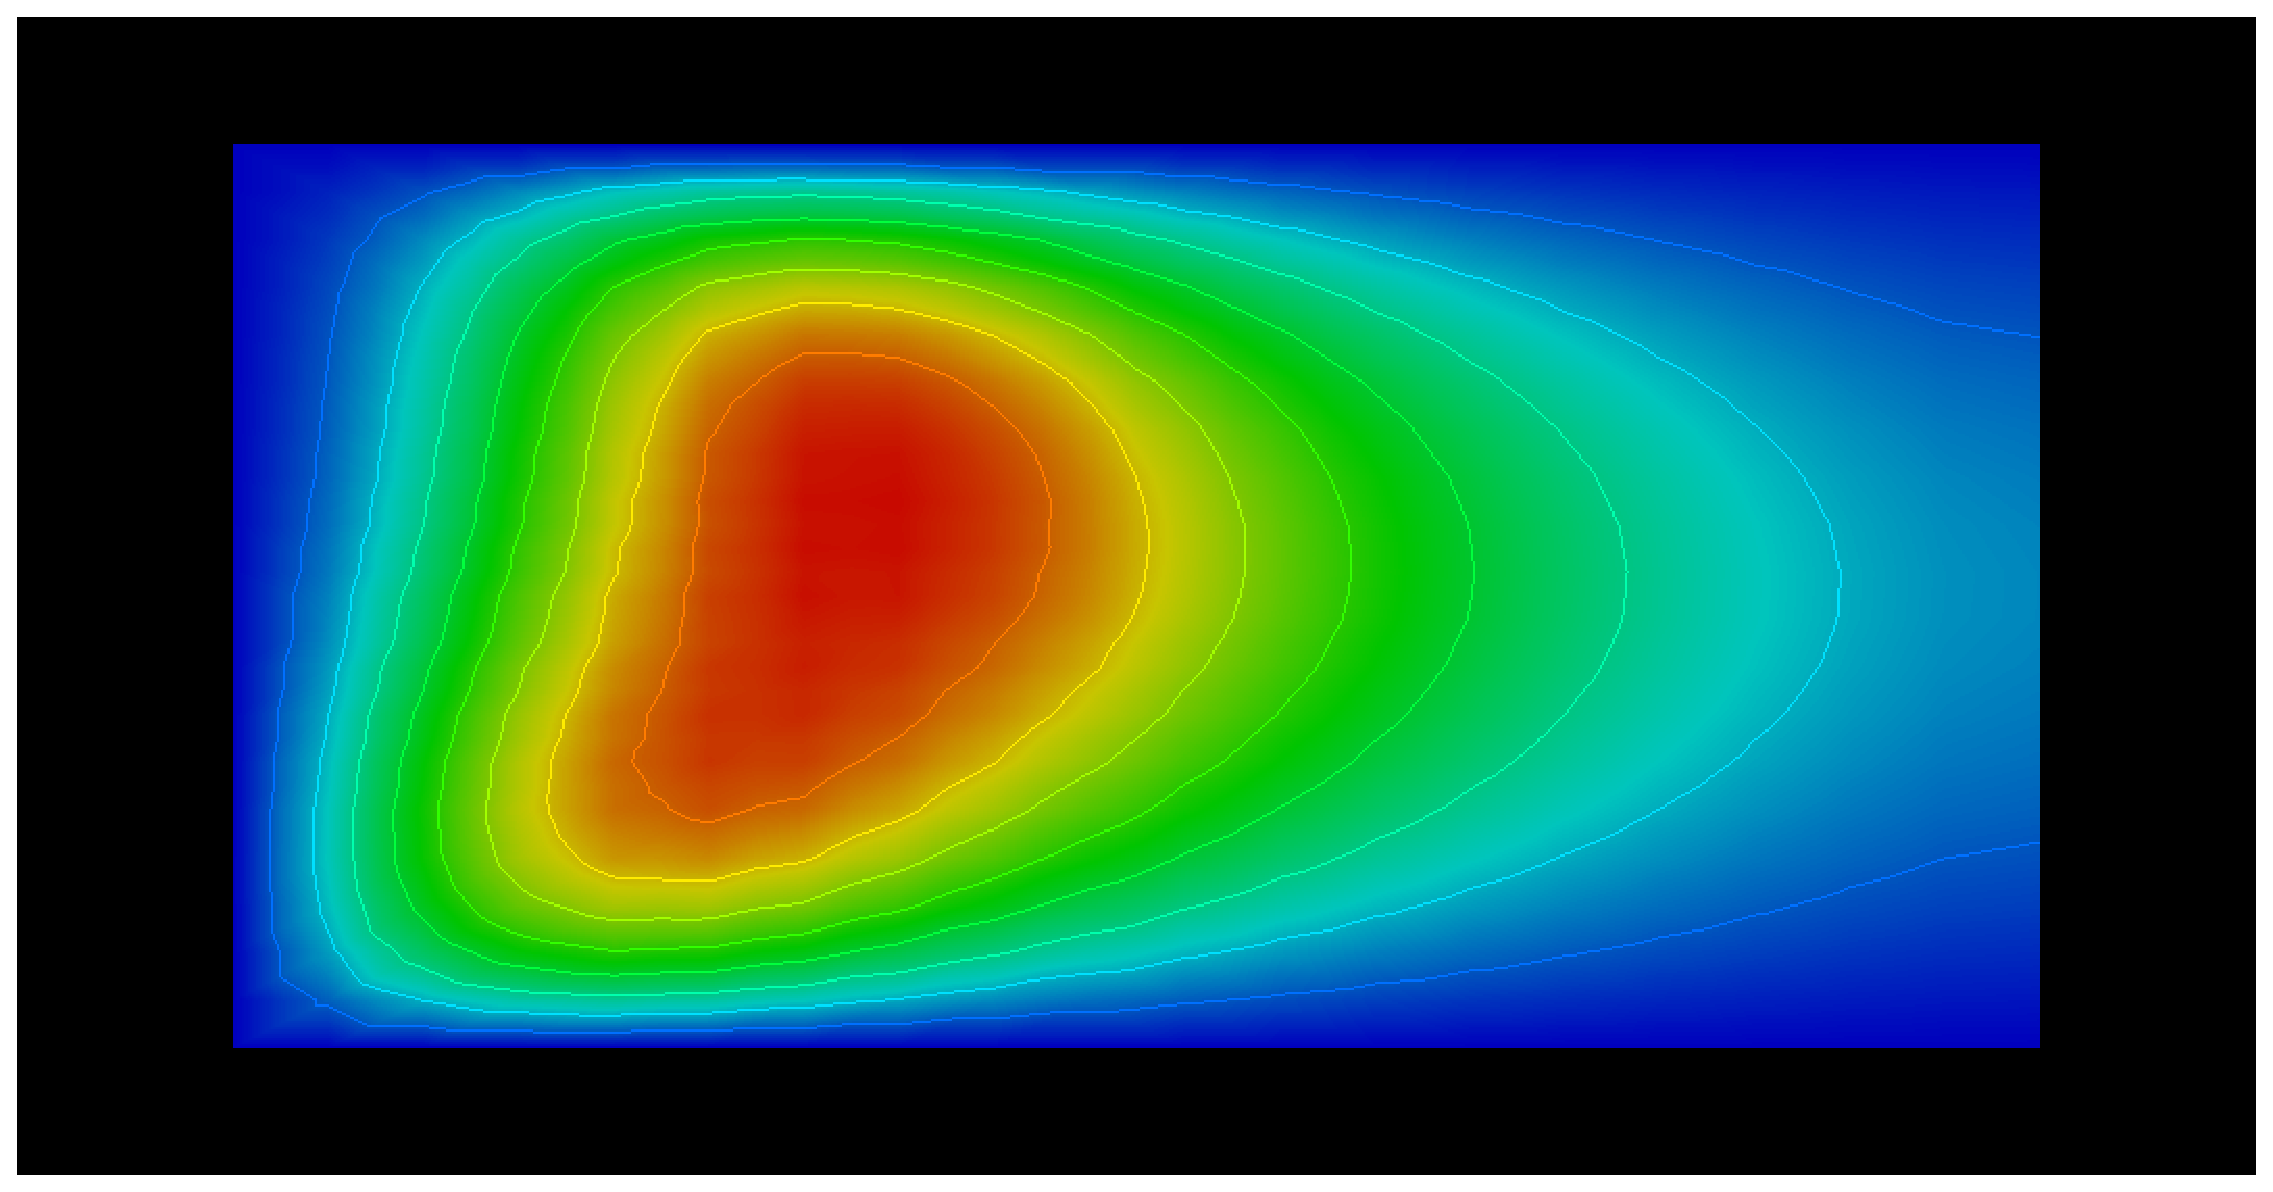
\includegraphics[scale=0.15]{DDDD_ADR/FEMslice.eps}}\qquad
        \caption{Caso test DDDD sezione XZ}
        \label{fig:DDDD_ADR slice}
\end{figure}

\begin{figure}[!htbp]
        \centering%
                \subfigure[Forzante e trasporto.]%
          {\label{fig: force term}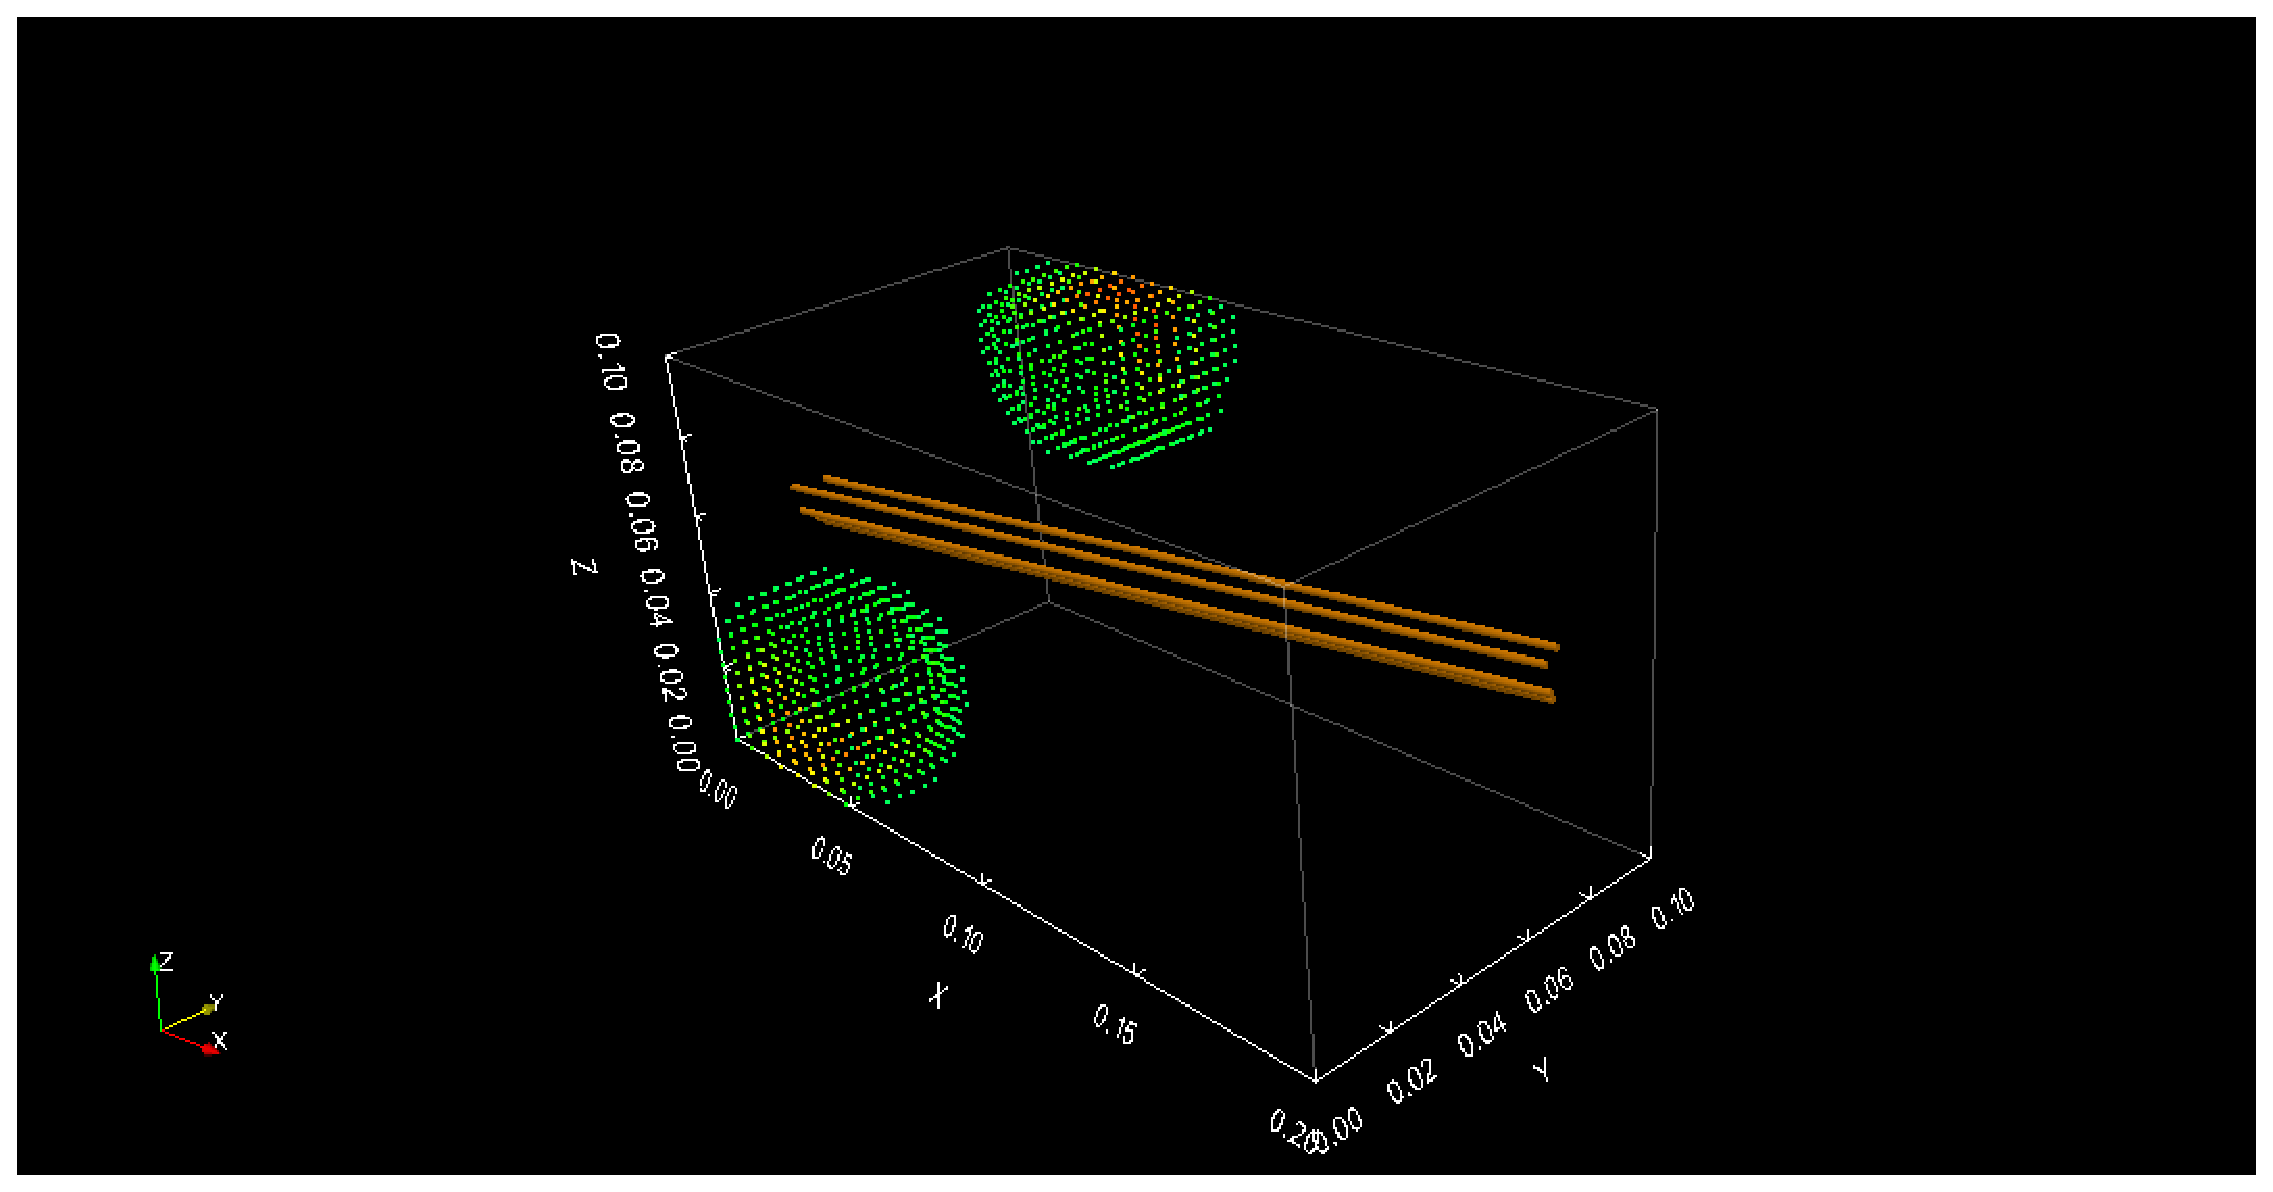
\includegraphics[scale=0.36]{DDDD_ADR/ForcetermTrasport.eps}}\qquad
        \subfigure[Soluzione FEM.]%
          {\label{fig: FEMsol}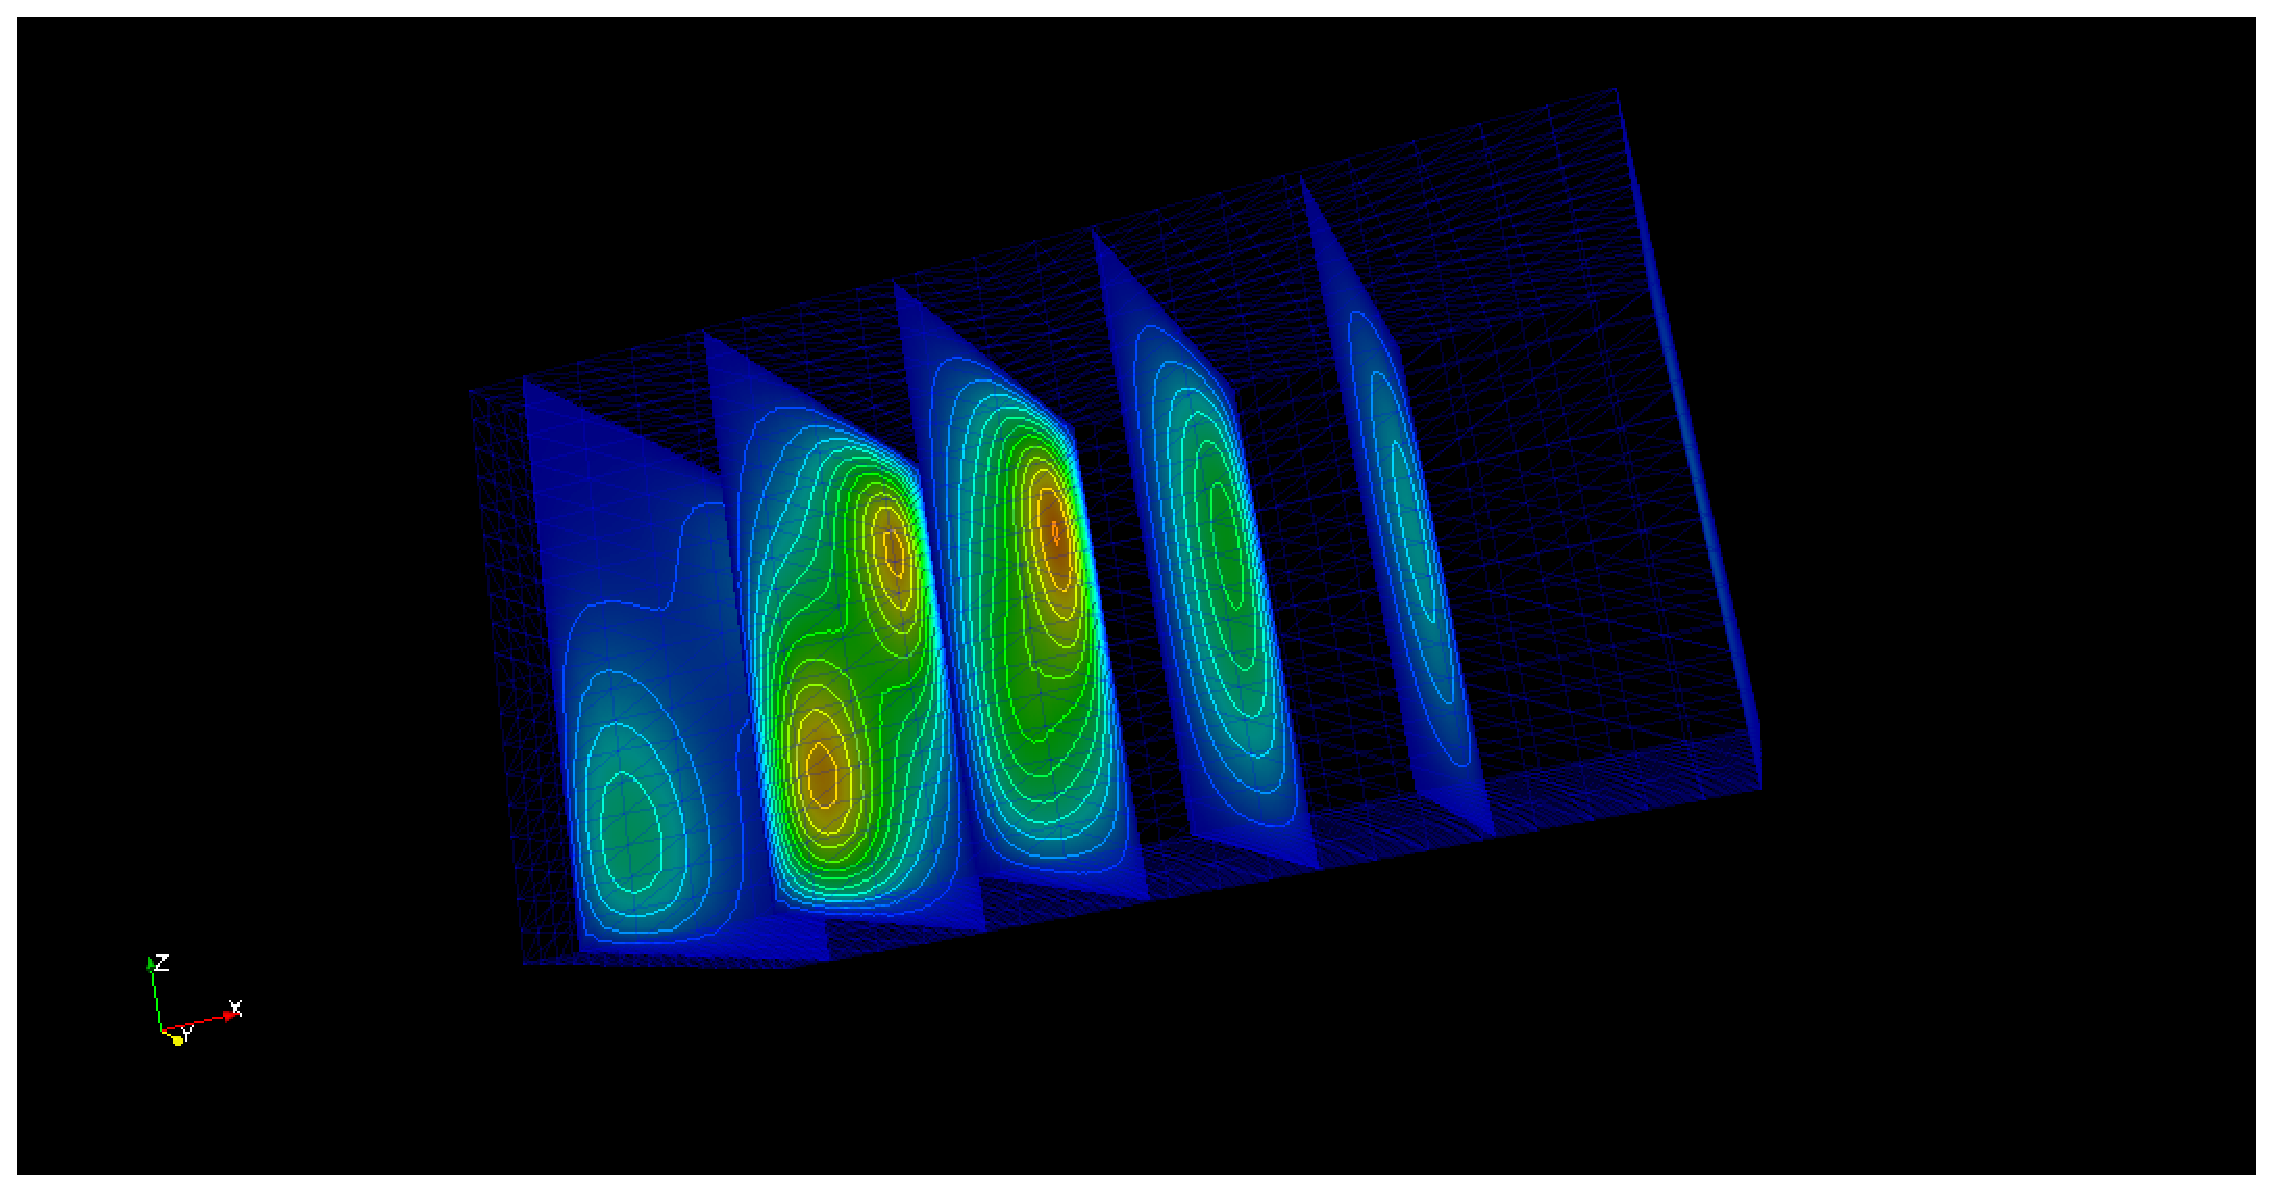
\includegraphics[scale=0.36]{DDDD_ADR/FEM.eps}}\qquad
        \subfigure[Soluzione HiMod m=50.]%
          {\label{fig:HiMod50sol}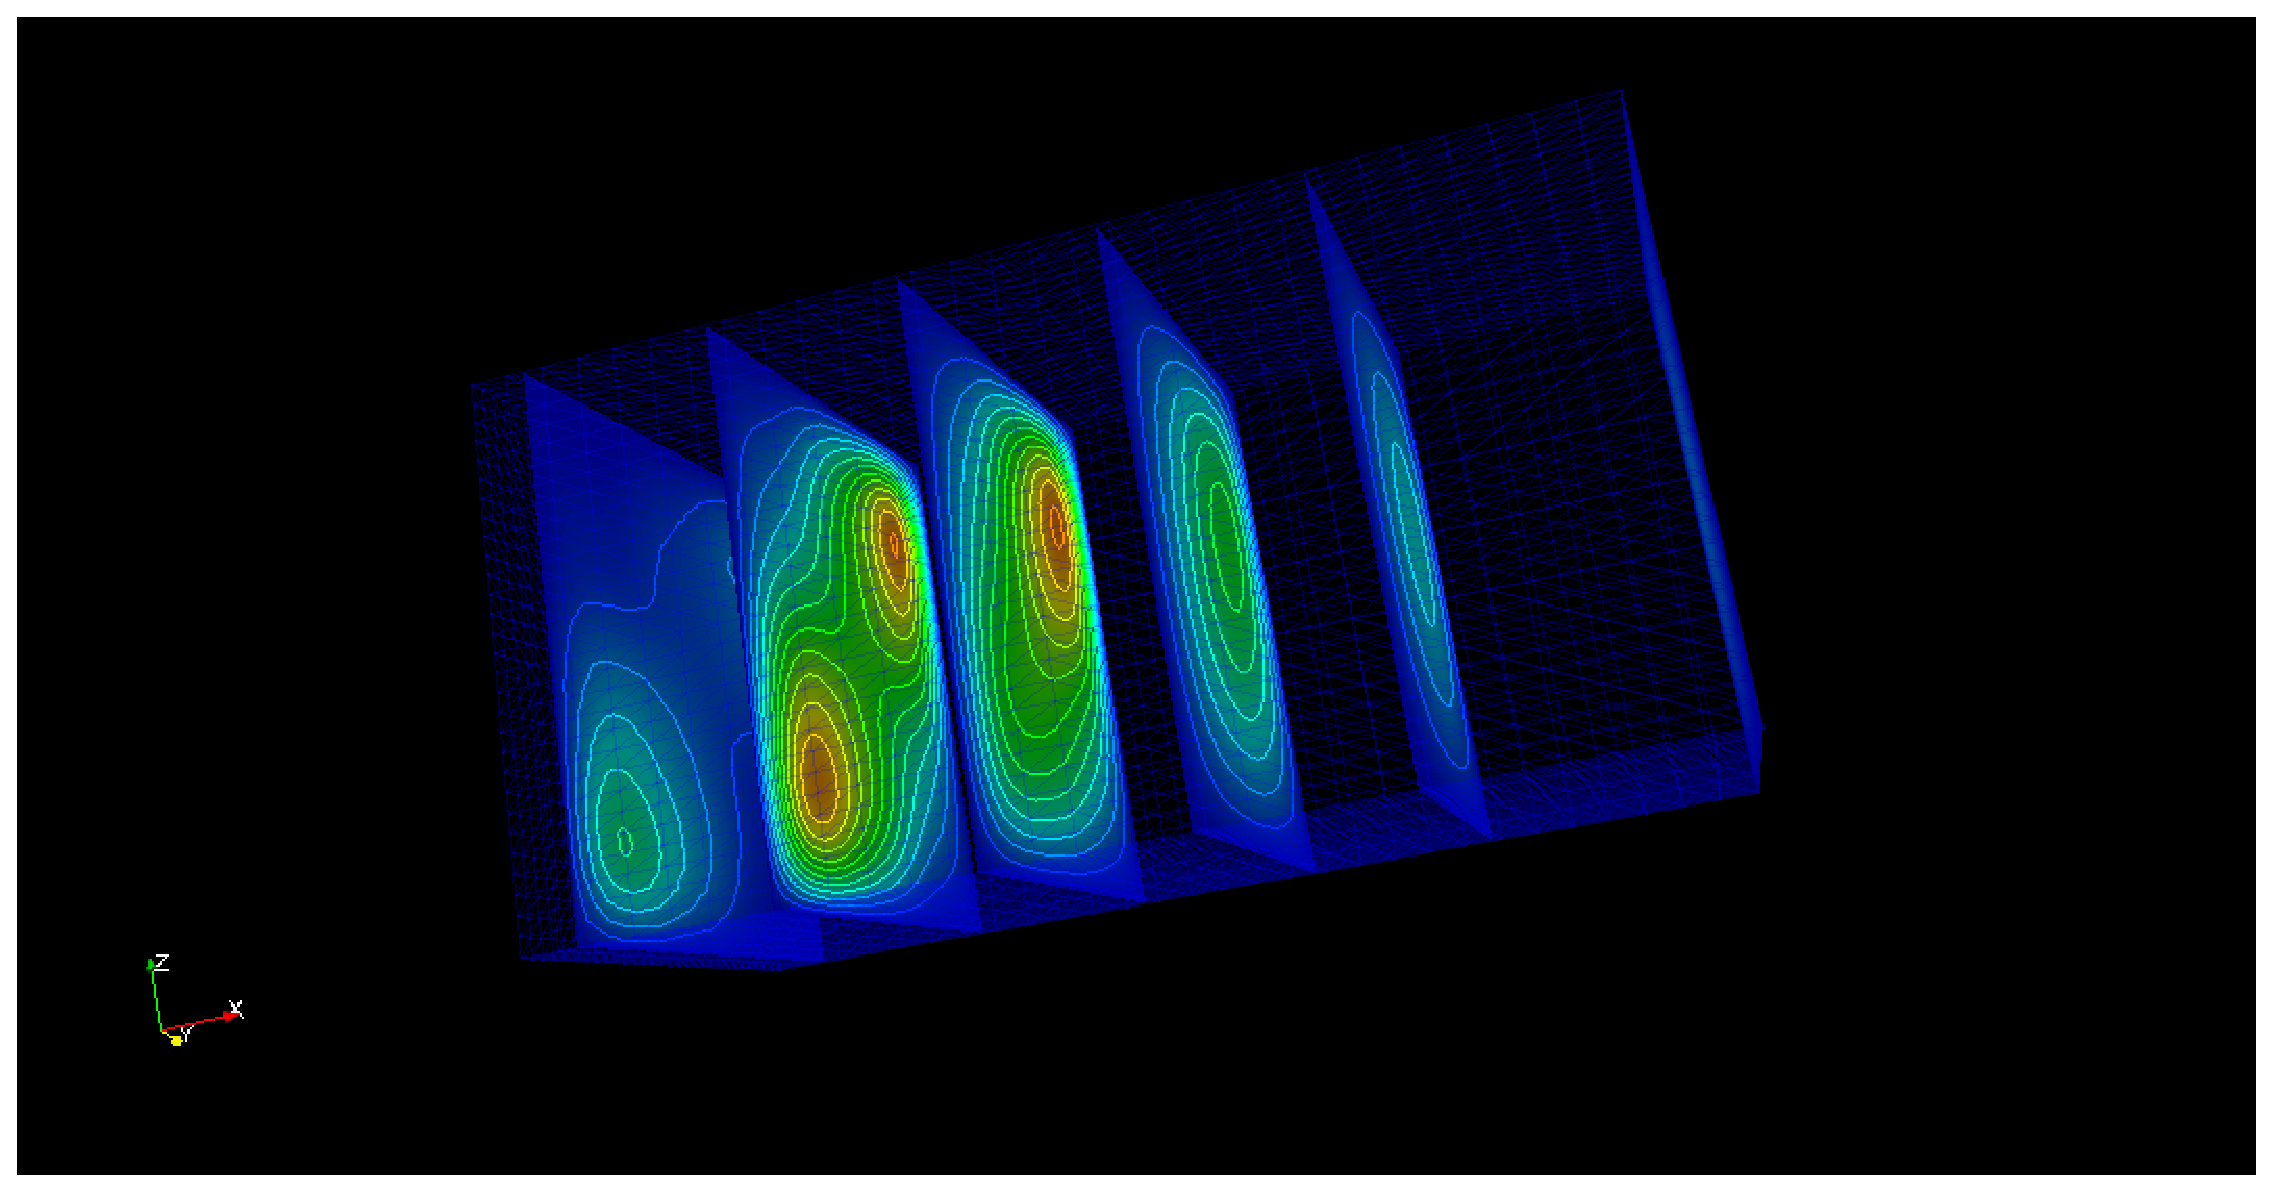
\includegraphics[scale=0.36]{DDDD_ADR/HiMod50.eps}}\qquad
        \caption{Caso test DDDD\_ADR}
        \label{fig:DDDD_ADR}
\end{figure}